\section{Durchführung}
\label{sec:Durchführung}
Die Messaperatur wird wie in \autoref{fig:schemaaufbau} aufgebaut. Zunächst wird eine $900 \unit{\second}$ lange Nullmessung durchgeführt, um die Hintergrundstrahlung zu ermitteln.
Danach wird ein $\gamma- \text{Strahler}$ Apparatur gesetzt. In diesem Fall wird eine Cs-137 Probe verwendet. Danach wird eine Blei Abschirmung zwischen Quelle und Geiger-Müller-Zählrohr eingesetzt. Für die Messreihe wird die Dicke der Abschirmung variiert und die Aktivität wird gemessen.

Für eine zweite Messreihe wird die Blei Abschirmung durch eine aus Kupfer ausgetauscht. Die Messdauer wird an die Dicke der Abschirmung angepasst. Für dicke Abschirmungen wird länger gemessen, damit die statistischen Schwankungen minimiert werden.

Das gleiche Experiment wird mit einem $\beta^{-}$- Strahler ersetzt und erneut eine Nullmessung durchgeführt. Bei dem zweiten Experiment ist die Quelle Tc-99 und die Abschirmung sind Aluminiumplatten.


\begin{figure}[h]
    \centering
    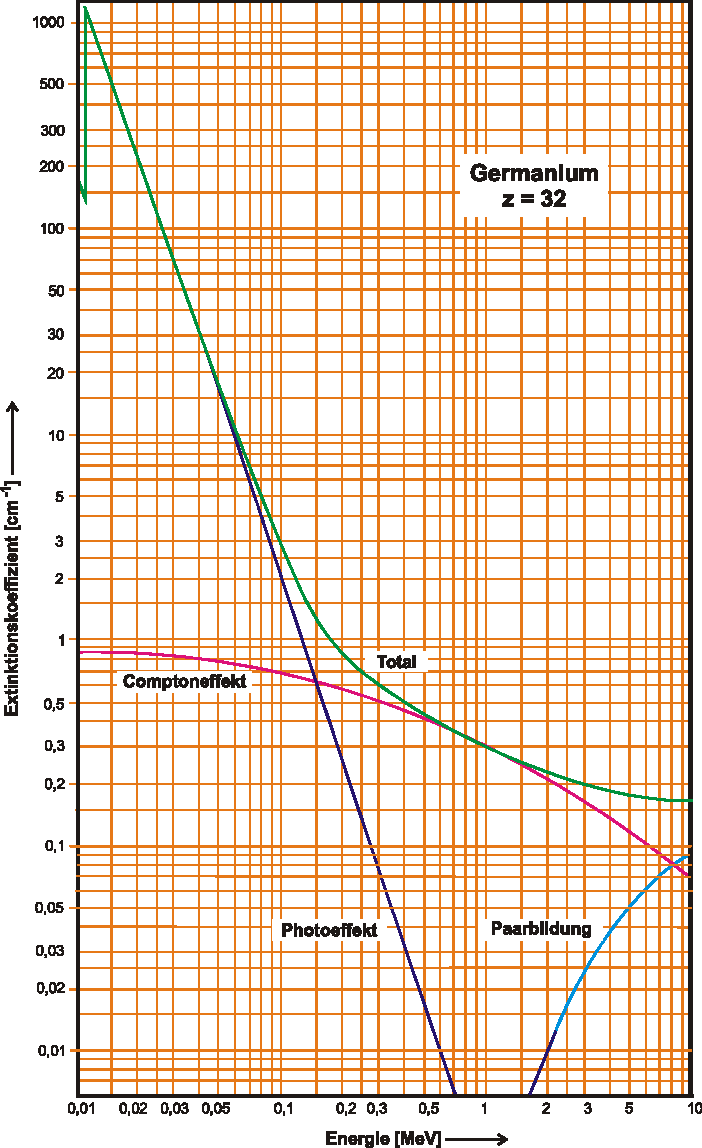
\includegraphics{figures/abb4.pdf}
    \caption{Schematische der Messaperatur \cite{ap04}.} 
    \label{fig:schemaaufbau}
\end{figure}